\notechapter{N-20261020}{Almost Nowhere, Yet Everywhere}

Can a subset of the real line have measure zero, intersect every open interval, and still deserve to be called \emph{typical}? We will construct one that does. Then we will construct a closed set with positive measure and no interior, and discover that these are only the beginning of the disagreement between two notions of size.

One way of describing a small set is to ask how much length it occupies. Another is to ask whether it leaves an open region in which it is absent, and whether it can be built by combining sets with that property. The first leads to Lebesgue measure; the second leads to Baire category. They support remarkably similar theorems and sometimes pronounce opposite verdicts on the very same subset of \(\mathbb R\). The classical source for this subject is Oxtoby's \emph{Measure and Category}, especially its opening chapters on the real line and Liouville numbers.\footnote{John C. Oxtoby, \href{https://link.springer.com/book/10.1007/978-1-4684-9339-9}{\emph{Measure and Category: A Survey of the Analogies between Topological and Measure Spaces}}, 2nd ed., Graduate Texts in Mathematics 2 (1980).}

I have a rather silly history with this little book. When I was much younger, I was so taken with Springer's Graduate Texts in Mathematics that I wanted the small personal triumph of finishing \emph{one whole GTM}. I chose GTM~2, partly because Oxtoby's volume looked like one of the thinnest on the shelf. The title made the bargain even sweeter: \emph{Measure and Category} sounded to me like a remarkably fancy pocket-sized tour of measure theory \emph{and} category theory. Well, it turns out that this category is Baire's category---meager sets, nowhere-dense sets, and all that---rather than the world of objects, arrows, and functors. Seven years later, opening the same slender volume again feels a little like meeting an old accomplice in a very innocent mathematical misunderstanding. At least this time I know what the title means.

Just to settle the misunderstanding properly, here are the two meanings side by side.

\begin{definition}[Baire category]
Let \(X\) be a topological space. A subset \(A\subseteq X\) is \emph{nowhere dense} if
\[
 \operatorname{int}_X(\overline A)=\varnothing.
\]
It is of \emph{first category}, or \emph{meager}, if it is a countable union of nowhere-dense subsets of \(X\); otherwise it is of \emph{second category}. A subset is \emph{comeager} (or \emph{residual}) if its complement is meager.
\end{definition}

\begin{definition}[Category in category theory]
A \emph{category} \(\mathcal C\) consists of a collection of objects, sets of morphisms \(\operatorname{Hom}_{\mathcal C}(A,B)\) for each pair of objects, identity morphisms \(\operatorname{id}_A:A\to A\), and associative composition
\[
 \operatorname{Hom}_{\mathcal C}(B,C)\times
 \operatorname{Hom}_{\mathcal C}(A,B)
 \longrightarrow \operatorname{Hom}_{\mathcal C}(A,C).
\]
Composition satisfies \(h\circ(g\circ f)=(h\circ g)\circ f\) whenever defined, and \(\operatorname{id}_B\circ f=f=f\circ\operatorname{id}_A\) for every \(f:A\to B\).
\end{definition}

\section{The Cantor set is already quite strange}

Start with the interval \(C_0=[0,1]\). Remove its open middle third to obtain
\[
 C_1=[0,\tfrac13]\cup[\tfrac23,1].
\]
From each of these two intervals remove its open middle third. Continue forever, and write \(C_n\) for the \(n\)th surviving set:
\[
 C=\bigcap_{n=0}^\infty C_n.
\]
At stage \(n\), \(C_n\) consists of \(2^n\) closed intervals, each of length \(3^{-n}\). Thus
\[
 \lambda(C_n)=2^n3^{-n}=\left(\frac23\right)^n,
 \qquad
 \boxed{\lambda(C)=0}.
\]
The last equality follows from continuity of measure from above, since \(C_0\) has finite measure. The set \(C\) is closed as an intersection of closed sets.

Yet \(C\) is uncountable. Every binary sequence \(b=(b_1,b_2,\ldots)\) determines a point
\[
 x_b=\sum_{n=1}^\infty\frac{2b_n}{3^n}\in C.
\]
Different binary sequences give different points: at the first place where two sequences differ, the discrepancy \(2\cdot3^{-n}\) exceeds the greatest possible contribution \(3^{-n}\) from all later terms. This gives an injection \(\{0,1\}^{\mathbb N}\hookrightarrow C\). A zero-measure set may contain uncountably many points.

There is a different sense in which \(C\) is small. It contains no nonempty open interval. If an interval \(I\subseteq C\) existed, then for large \(n\) it would have to fit inside a component of \(C_n\), each of which has length \(3^{-n}<|I|\), an impossibility. Since \(C\) is closed, this says that \(C\) is \emph{nowhere dense}:
\[
 \operatorname{int}\overline C=\varnothing.
\]
A nowhere-dense set is one whose closure fails to contain even one nonempty open interval. Notice that it can still have many accumulation points; indeed the Cantor set is perfect, with no isolated points.

\begin{figure}[htbp]
\centering
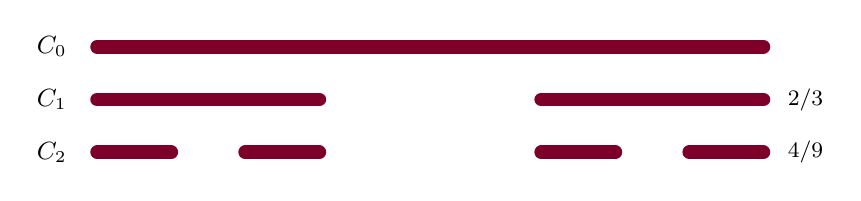
\begin{tikzpicture}[x=.94cm,y=.67cm,line cap=round,
 every node/.style={font=\small}]
 \node[anchor=east] at (-.28,2) {\(C_0\)};
 \node[anchor=east] at (-.28,1) {\(C_1\)};
 \node[anchor=east] at (-.28,0) {\(C_2\)};
 \draw[line width=5pt,purple!65!black] (0,2)--(9,2);
 \foreach \a/\b in {0/3,6/9}{
  \draw[line width=5pt,purple!65!black] (\a,1)--(\b,1);
 }
 \foreach \a/\b in {0/1,2/3,6/7,8/9}{
  \draw[line width=5pt,purple!65!black] (\a,0)--(\b,0);
 }
 \node[anchor=west,font=\footnotesize] at (9.2,1) {\(2/3\)};
 \node[anchor=west,font=\footnotesize] at (9.2,0) {\(4/9\)};
\end{tikzpicture}
\caption{The first two deletions in the middle-thirds Cantor construction. After \(n\) stages, \(2^n\) short intervals remain, while their total length decays as \((2/3)^n\).}
\label{fig:N20261020-cantor}
\end{figure}

\section{A fat Cantor set}

Could the deletion scheme leave a set with \emph{positive} measure, yet still no interior? Yes. Keep the left-right splitting procedure but remove less length.

Begin again with \(F_0=[0,1]\). At stage \(n\geq1\), remove from the middle of each of the \(2^{n-1}\) surviving closed intervals an open interval of length \(4^{-n}\). The first stage removes an interval of length \(1/4\); the second removes two intervals of length \(1/16\); the third removes four intervals of length \(1/64\), and so forth. Define \(F=\bigcap_{n=0}^\infty F_n\).

There is room for all these deletions. At stage \(n-1\), each of the \(2^{n-1}\) remaining intervals has the same length
\[
 \ell_{n-1}
 =\frac{1-\sum_{k=1}^{n-1}2^{k-1}4^{-k}}{2^{n-1}}
 =\frac{1/2+2^{-n}}{2^{n-1}},
\]
which is strictly greater than the next deletion length \(4^{-n}\).

The total removed length is
\[
 \sum_{n=1}^\infty2^{n-1}4^{-n}
 =\sum_{n=1}^\infty2^{-n-1}=\frac12.
\]
Because the deleted intervals are disjoint,
\[
 \boxed{\lambda(F)=\frac12}.
\]
Each component of \(F_n\) has length at most \(2^{-n}\). For every interval \(I\) of positive length, sufficiently late components are shorter than \(I\), so \(I\not\subseteq F\). The set \(F\) is closed with empty interior: it is nowhere dense and occupies exactly half the unit interval.

\begin{figure}[htbp]
\centering
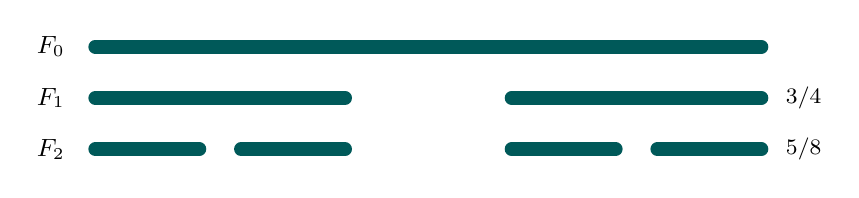
\begin{tikzpicture}[x=.94cm,y=.65cm,line cap=round,
 every node/.style={font=\small}]
 \node[anchor=east] at (-.28,2) {\(F_0\)};
 \node[anchor=east] at (-.28,1) {\(F_1\)};
 \node[anchor=east] at (-.28,0) {\(F_2\)};
 \draw[line width=5pt,teal!70!black] (0,2)--(9,2);
 \draw[line width=5pt,teal!70!black] (0,1)--(3.375,1);
 \draw[line width=5pt,teal!70!black] (5.625,1)--(9,1);
 \foreach \a/\b in {0/1.40625,1.96875/3.375,5.625/7.03125,7.59375/9}{
  \draw[line width=5pt,teal!70!black] (\a,0)--(\b,0);
 }
 \node[anchor=west,font=\footnotesize] at (9.2,1) {\(3/4\)};
 \node[anchor=west,font=\footnotesize] at (9.2,0) {\(5/8\)};
\end{tikzpicture}
\caption{The first two stages of a Smith--Volterra--Cantor construction. It has the same endlessly branching structure as the previous set, but its total remaining length tends to \(1/2\).}
\label{fig:N20261020-fatcantor}
\end{figure}

We could have made the retained measure as close to \(1\) as desired. For \(0<\varepsilon<1\), remove length \(2\varepsilon\,4^{-n}\) from the middle of each surviving interval at stage \(n\). The total removed length is
\[
 \sum_{n\geq1}2^{n-1}(2\varepsilon\,4^{-n})=\varepsilon.
\]
The resulting closed nowhere-dense set has measure \(1-\varepsilon\). Thus nowhere density places no useful upper bound on Lebesgue measure below the measure of the whole interval.

The two Cantor-type sets have brought us to a question. A nowhere-dense set is small in the topology of open intervals, whether its measure is \(0\), \(1/2\), or \(0.999\). What happens if we allow \emph{countably many} nowhere-dense pieces?

\section{Completeness and the Baire theorem}

A set \(A\) is \emph{meager} (of first category) if it is a countable union of nowhere-dense sets, or is contained in such a union. A set is \emph{comeager} or \emph{residual} if its complement is meager. Here category is Baire's classical terminology; it has no connection with the notion of a category in homological algebra or category theory.

Finite unions of nowhere-dense sets are nowhere dense. A countable union is a different matter. Every singleton \(\{q\}\subseteq\mathbb R\) is nowhere dense, so the rational numbers
\[
 \mathbb Q=\bigcup_{q\in\mathbb Q}\{q\}
\]
are meager. But \(\mathbb Q\) is dense in \(\mathbb R\). Being nowhere dense is not a property preserved under a countable union.

Could all of \(\mathbb R\) be obtained as a countable union of nowhere-dense sets? The Baire category theorem rules that out.

\begin{theorem}[Baire category theorem]
If \((X,d)\) is a complete metric space and \(U_1,U_2,\ldots\) are open dense subsets of \(X\), then
\[
 \bigcap_{n=1}^\infty U_n
\]
is dense in \(X\). In particular, every nonempty open subset of \(X\) is nonmeager in itself.
\end{theorem}

\begin{proof}
Let \(W\subseteq X\) be an arbitrary nonempty open set. We must find a point of \(W\) belonging to every \(U_n\).

Because \(U_1\) is open and dense, \(W\cap U_1\) is nonempty and open. Choose a closed ball
\[
 \overline{B_1}=\overline{B}(x_1,r_1)
 \subseteq W\cap U_1,\qquad 0<r_1<\frac12.
\]
The open set \(B_1\cap U_2\) is also nonempty. Choose a second closed ball
\[
 \overline{B_2}\subseteq B_1\cap U_2,\qquad0<r_2<\frac14.
\]
Continue, choosing
\[
 \overline{B_{n+1}}\subseteq B_n\cap U_{n+1},
 \qquad0<r_{n+1}<2^{-n-1}.
\]
The closed balls are nested, and their diameters tend to zero. Their centers form a Cauchy sequence: if \(m>n\), then \(x_m\in B_n\), so \(d(x_m,x_n)\le r_n\). Completeness gives a limit \(x\in X\).

For each fixed \(n\), all later centers belong to \(\overline{B_n}\), a closed set, so \(x\in\overline{B_n}\). Hence \(x\in U_n\) for every \(n\) and \(x\in W\). Since \(W\) was arbitrary, the intersection is dense.
\end{proof}

The key geometric action is to keep choosing a smaller closed ball inside a new open dense set. The radii go to zero, and completeness guarantees that this infinite sequence of compatible choices still leaves an actual point. Without completeness, the procedure may converge to a point missing from the space: \(\mathbb Q\), with its usual metric, is itself a countable union of nowhere-dense singletons.

A set of the form \(\bigcap_n U_n\), where the \(U_n\) are open, is called a \(G_\delta\) set. A countable intersection of \emph{open dense} sets is a particularly useful kind of \(G_\delta\): Baire's theorem says it remains dense. Moreover any countable intersection of dense \(G_\delta\) sets is dense \(G_\delta\), since we may collect all the open dense factors into one countable family.

\section{A set that is negligible and generic}

We are ready for the most conspicuous disagreement between measure and category. First enumerate the rationals as
\[
 \mathbb Q=\{q_1,q_2,\ldots\}.
\]
For every \(n\ge1\), place a tiny interval around each rational and take their union:
\begin{equation}
 V_n=\bigcup_{j=1}^\infty
 \left(q_j-2^{-n-j-2},\,q_j+2^{-n-j-2}\right).
 \label{eq:N20261020-tiny-open}
\end{equation}
Each \(V_n\) is open and contains all rationals, so it is dense. Yet a countable subadditivity calculation gives
\[
 \lambda(V_n)
 \leq\sum_{j=1}^\infty 2^{-n-j-1}
 =2^{-n-1}.
\]
Thus \(V_n\) is open and dense while occupying a very small total length. As \(n\) grows, this length shrinks to zero.

Consider the set
\[
 G=\bigcap_{n=1}^\infty V_n.
\]
By Baire's theorem, \(G\) is dense \(G_\delta\); in particular it is comeager. But \(G\subseteq V_n\) for every \(n\), so
\[
 0\leq\lambda(G)\leq\inf_n2^{-n-1}=0.
\]
We have constructed
\begin{equation}
 \boxed{\text{\(G\) is comeager and dense, yet \(\lambda(G)=0\).}}
 \label{eq:N20261020-residual-null}
\end{equation}
Its complement \(H=\mathbb R\setminus G\) is meager, since it is the union of the nowhere-dense closed sets \(\mathbb R\setminus V_n\). Meanwhile
\[
 \lambda(\mathbb R\setminus H)=\lambda(G)=0.
\]
Thus \(H\) has \emph{full Lebesgue measure}, in the sense that its complement is null, even though \(H\) is meager. Both \(G\) and \(H\) are dense: every nonempty open interval has positive length and cannot be contained in the null set \(G\).

Here is a precise answer to the opening question. The statement that a property holds \emph{almost everywhere} means that its failure set has measure zero. The statement that it holds \emph{generically} in the Baire sense means that its failure set is meager. On the real line these two notions can make opposite claims about the same property.

A concrete property having this behavior is waiting for us in number theory.

\section{Numbers that are exceptionally easy to approximate}

A real number \(x\) is a \emph{Liouville number} if it can be approximated by rational numbers to an arbitrarily high algebraic order: for every integer \(k\ge1\) and every \(N\ge2\), there exist integers \(p\) and \(q\ge N\) such that
\begin{equation}
 0<\left|x-\frac pq\right|<\frac1{q^k}.
 \label{eq:N20261020-Liouville}
\end{equation}
The requirement that the inequality hold for arbitrarily large denominators rules out merely repeating a single rational approximation. It is equivalent to the usual Liouville condition for irrational \(x\), with the additional insistence that \(x\) itself is not rational.

There are explicit examples. Take
\[
 L=\sum_{j=1}^\infty10^{-j!}
  =0.110001000000000000000001\ldots
\]
and its rational truncations \(L_m=\sum_{j=1}^{m}10^{-j!}\). The denominator of \(L_m\) is \(q_m=10^{m!}\); the omitted tail is bounded by
\[
 0<L-L_m<2\cdot10^{-(m+1)!}
       =2q_m^{-(m+1)}.
\]
For any prescribed \(k\), choose \(m\) so large that \(m+1>k\) and \(2q_m^{-(m+1)}<q_m^{-k}\). This exhibits rational approximations satisfying \eqref{eq:N20261020-Liouville} with denominators tending to infinity.

Why are these numbers called especially well approximated? Suppose instead that \(\alpha\) is algebraic of degree \(d\), with a nonzero polynomial \(P\in\mathbb Z[x]\) of degree \(d\) satisfying \(P(\alpha)=0\). For any rational \(p/q\ne\alpha\), where \(q\ge1\),
\[
 q^dP(p/q)\in\mathbb Z\setminus\{0\},
 \qquad |P(p/q)|\ge q^{-d}.
\]
If \(p/q\) is near \(\alpha\), the derivative \(P'\) is bounded by some constant \(M>0\) on the interval between them. The mean value theorem gives
\[
 |P(p/q)|
 =|P(p/q)-P(\alpha)|
 \le M|p/q-\alpha|.
\]
Therefore
\begin{equation}
 \left|\alpha-\frac pq\right|
 \ge\frac1{Mq^d}.
 \label{eq:N20261020-algebraic-bound}
\end{equation}
For sufficiently large \(q\), this contradicts a requirement such as
\(|\alpha-p/q|<q^{-(d+1)}\). Consequently every Liouville number is transcendental.

This establishes an unexpected kind of rarity, but the measure and category of the \emph{whole set} of Liouville numbers are even more interesting.

\section{The Liouville numbers form a dense null \(G_\delta\)}

For integers \(k\ge1\) and \(N\ge2\), define
\begin{equation}
 U_{k,N}
 =\bigcup_{\substack{q\ge N\\p\in\mathbb Z}}
 \left(
 \left(\frac pq-q^{-k},\frac pq\right)
 \cup
 \left(\frac pq,\frac pq+q^{-k}\right)
 \right).
 \label{eq:N20261020-Ukn}
\end{equation}
This is open. It is also dense: for every open interval \(I\), choose a sufficiently large denominator \(q\) and a rational \(p/q\) strictly inside \(I\); points immediately to either side of \(p/q\) also lie in \(I\cap U_{k,N}\). The set \(\mathcal L\) of Liouville numbers is exactly
\begin{equation}
 \mathcal L
 =\bigcap_{k=1}^\infty\bigcap_{N=2}^\infty U_{k,N}.
 \label{eq:N20261020-Liouville-Gdelta}
\end{equation}
It is a countable intersection of open dense subsets of \(\mathbb R\). Therefore Baire's theorem says that \(\mathcal L\) is a dense \(G_\delta\) set, hence comeager.

To prove it has measure zero, fix \(R>0\), and consider \(U_{4,N}\cap[-R,R]\). If one of the intervals centered at \(p/q\) meets \([-R,R]\), then for \(q\ge2\) we have \(|p/q|\le R+1\). For each \(q\), at most \(2(R+1)q+3\) integers \(p\) have this property, and each punctured interval has total length \(2q^{-4}\). Hence, for a constant \(K_R\) independent of \(N\),
\[
 \lambda(U_{4,N}\cap[-R,R])
 \le K_R\sum_{q=N}^\infty q^{-3}
 \xrightarrow[N\to\infty]{}0.
\]
But \(\mathcal L\subseteq U_{4,N}\) for every \(N\); thus
\[
 \lambda(\mathcal L\cap[-R,R])=0
 \qquad\text{for every }R>0.
\]
Taking a countable union of such bounded intervals yields
\begin{equation}
 \boxed{\lambda(\mathcal L)=0,\qquad
        \mathcal L\text{ is dense and comeager in }\mathbb R.}
 \label{eq:N20261020-Liouville-contrast}
\end{equation}
In fact the complement \(\mathbb R\setminus\mathcal L\) has full Lebesgue measure while being meager. Almost every real number is \emph{not} a Liouville number, and a Baire-generic real number \emph{is} a Liouville number.

The result goes further than a curious classification of sets. It gives a very short proof of a remarkable statement about addition.

\begin{proposition}
Every real number is the sum of two Liouville numbers. Equivalently,
\[
 \mathcal L+\mathcal L=\mathbb R.
\]
\end{proposition}
\begin{proof}
Fix \(t\in\mathbb R\). Since \(\mathcal L\) is dense \(G_\delta\), so is the translate and reflection \(t-\mathcal L=\{t-y:y\in\mathcal L\}\). To see this directly, apply the homeomorphism \(x\mapsto t-x\) to each open dense set in \eqref{eq:N20261020-Liouville-Gdelta}. By Baire's theorem,
\[
 \mathcal L\cap(t-\mathcal L)\ne\varnothing.
\]
Choose \(x\) in this intersection. Then \(x\in\mathcal L\) and \(t-x\in\mathcal L\), giving \(t=x+(t-x)\).
\end{proof}

Every Liouville number is transcendental, so even \emph{every algebraic number} can be written as the sum of two particular transcendental numbers. A measure-zero subset of the line has sumset equal to the entire line. Cardinality and length cannot predict this additive behavior; category provides an elegant existence proof.

\section{What does a homeomorphism remember?}

There is a second reason to separate topology from measure. The two Cantor-type sets we constructed at the beginning are actually \emph{homeomorphic}. To see this without a classification theorem, label the left and right surviving intervals at each stage by \(0\) and \(1\). An infinite binary sequence \(b=(b_1,b_2,\ldots)\) singles out one nested sequence of intervals in \(C\), hence one point \(c_b\). The same sequence singles out one point \(f_b\) of the fat Cantor set \(F\).

Both interval trees shrink in diameter to zero, so the correspondence \(c_b\mapsto f_b\) is continuous, bijective and has a continuous inverse. It preserves order: if two binary sequences first differ at position \(n\), the point with digit \(0\) lies to the left of the point with digit \(1\) in both constructions.

In fact it extends to an increasing homeomorphism
\[
 h:[0,1]\longrightarrow[0,1],
 \qquad h(C)=F.
\]
Each complementary interval of \(C\) corresponds, under the left-right address system, to one complementary interval of \(F\). Map their endpoints accordingly, and extend the map linearly across each gap. The resulting strictly increasing function is continuous, fixes \(0,1\), and therefore has a continuous inverse.

We have produced a homeomorphism with
\[
 \lambda(C)=0,\qquad
 \lambda(h(C))=\lambda(F)=\frac12.
\]
Thus Lebesgue measure zero is \emph{not} invariant under arbitrary homeomorphisms. In contrast, homeomorphisms preserve the property of being nowhere dense, since they preserve closures and interiors, and therefore preserve meager and comeager sets.

There is a useful boundary on the example. If a map \(h:[0,1]\to\mathbb R\) is \(K\)-Lipschitz, then it maps Lebesgue-null sets to Lebesgue-null sets. Indeed, cover a null set \(A\) by intervals \(I_j\) with \(\sum_j|I_j|<\varepsilon\). Every image \(h(I_j)\) is contained in an interval of length at most \(K|I_j|\), and so
\[
 \lambda^*(h(A))\le K\sum_j|I_j|<K\varepsilon.
\]
Letting \(\varepsilon\to0\) gives \(\lambda(h(A))=0\). Consequently the homeomorphism taking \(C\) to our fat Cantor set cannot be Lipschitz. Topological continuity allows deformations that quantitative regularity would forbid.

\section{Two different ways to ignore small sets}

Consider an open set \(U\subseteq\mathbb R\) and an open family \(U_i\subseteq U\). One way to call the family a cover is to require
\[
 \overline{\bigcup_iU_i}\supseteq U.
\]
This says that the union of the pieces is \emph{dense} in \(U\): there is no nonempty open part of \(U\) that the family completely misses.

Another way, given a measure \(\mu\), is to require
\[
 \mu\left(U\setminus\bigcup_iU_i\right)=0.
\]
This says that the family covers \(U\) \emph{almost everywhere}. Lafforgue's lecture on the measure-theoretic topology of language-model probability spaces uses this latter kind of measure-induced covering relation, and it is instructive to compare the two requirements in a familiar setting.

For Lebesgue measure on \((0,1)\), let \(F\) be the fat Cantor set of measure \(1/2\). The relative complement
\[
 V=(0,1)\setminus F
\]
is open and dense in \((0,1)\). But
\[
 \lambda(V)=\frac12<1=\lambda((0,1)).
\]
Thus the singleton family \(\{V\}\) covers \((0,1)\) in the dense-cover sense and fails to cover it in the almost-everywhere sense.

Conversely, if \(\lambda(U\setminus V)=0\) with \(V\) open in \(U\), then \(V\) must be dense in \(U\). Otherwise some nonempty open interval \(I\subseteq U\setminus\overline V\) would have positive measure and lie outside \(V\), a contradiction. For Lebesgue measure, almost-everywhere open coverage is therefore stronger than dense open coverage.

This implication relies on the fact that every nonempty open interval has positive Lebesgue measure. For a probability measure concentrated at one point, even that can fail. On \(X=[0,1]\), take \(\mu=\delta_0\) and the relatively open set \(V=[0,1/4)\). Then \(\mu(V)=\mu(X)=1\), but \(V\) is far from dense in \(X\).

The two covering rules discard different kinds of exceptional sets. In one, the missing pieces are invisible to the measure; in the other, the missing pieces have no open interior. The constructions in this chapter show why these are distinct mathematical judgements, even on the real line.
